\documentclass[11pt,a4paper]{article}
\usepackage[margin=2.35cm]{geometry}
\usepackage[T1]{fontenc}
\usepackage[utf8]{inputenc}
\usepackage{lmodern}
\usepackage{setspace}
\setstretch{1.16}
\setlength{\parskip}{0.35em}
\setlength{\parindent}{1em}
\usepackage{amsmath,amssymb}
\usepackage{booktabs}
\usepackage{tikz}
\usetikzlibrary{arrows.meta,positioning}
\usepackage[hidelinks]{hyperref}

\title{A Vision-Guided Feed-Speed Controller for a Wooden Seed Sowing Machine}
\author{}
\date{}

\begin{document}
\maketitle
\thispagestyle{empty}

\begin{abstract}
\noindent
Hardwood seeds such as acorns vary in diameter and lock against each other in a hopper throat. A meter that only tracks shaft speed will keep turning at the kinematic command while the throat is bridged, and the spacing error is then already committed. This short paper specifies a vision-guided feed-speed controller for that failure. A camera over the throat publishes occupancy, equivalent diameter, and a bridge index. The motor loop, on a separate computer, multiplies the kinematic shaft command by a scale that falls when the bridge index crosses a threshold, and a fuzzy proportional--integral--derivative law tracks the scaled command. The scale cut is capped, so one bad frame cannot stall the wheel. A numerical estimate of the same event model used in the parent thesis, not a field trial, shows the expected pattern: on red oak the multiple index falls from 22.5\% with speed tracking alone to 12.5\% with the constraint, while planting efficiency stays near 61\% because some spacings stretch. On bur oak and under a 16~Hz frame disturbance, slowing the feed without changing vibration does not repair the miss index. The controller is a quality intervention on doubles, with a rate side effect that must be reported separately.
\end{abstract}

\section{Introduction}

Direct seeding of oak can cost about a third of planting nursery seedlings, so the placement of each wooden seed is worth controlling \cite{lof2019}. The seed is a poor match to a cereal meter. Pin oak, red oak, and bur oak differ by more than the adjustment range of one cell, and two acorns readily form an arch. A ground wheel copies slip into every spacing. An electronic drive removes that slip by tracking
\begin{equation}
\omega^{\star} = \frac{2\pi v}{N_c X_t},
\label{eq:w}
\end{equation}
with $v$ the ground speed, $X_t$ the target spacing, and $N_c$ the number of cells \cite{he2017,zhao2024}. Tracking is not enough. If the throat is bridged, $\omega^{\star}$ is the speed at which empty cells are presented on time. The error the operator sees is a gap, and a tube sensor reports it only after the cell has passed \cite{kocher1998}.

Borja and colleagues put a camera on a corn plate and advanced the plate when a hole was empty \cite{borja2021}. Classification was accurate, and misses fell at 2 and 4~km/h. At 6~km/h misses rose, because one microcontroller could not finish the image and the motor update. The design in this paper keeps that lesson and changes the action. The camera does not classify plate holes of a graded seed. It compresses the throat of a wooden-seed meter into a bridge index, and the motor is allowed to slow down. Slowing is a decision, not a tracking error.

\section{Bridge index and the speed constraint}

The nominal machine is the single-row planter of the parent study: $N_c=12$, cell mouth $d_c=24$~mm, $X_t=0.25$~m, and forward speed near 0.7 to 1.1~m/s. At 1.10~m/s, Equation~\eqref{eq:w} asks for 22.0~r/min. The camera looks at a fixed window in the throat at 20~Hz. Otsu's threshold separates seed pixels from a stored empty-throat image \cite{otsu1979}. Components supply area and equivalent diameter $d=2\sqrt{A/\pi}$. Occupancy $\rho$ is seed area over window area. The bridge index is
\begin{equation}
B = \rho\,(0.45+0.55\min(1,c_d/0.25))\Big(1+\frac{\max(\bar d-d_c,0)}{d_c}\Big),
\label{eq:B}
\end{equation}
with $c_d$ the coefficient of variation of the diameters in view. Occupancy alone would treat a full but flowing throat as a bridge. The diameter term raises $B$ when the seeds are larger than the cell, which is the bur-oak case. A one-pole filter, $\rho\leftarrow 0.92\rho+0.08\rho_{\mathrm{raw}}$, stops one specular frame from slamming the wheel.

The constrained command is $\omega_{\mathrm{cmd}}=\sigma(B)\,\omega^{\star}$, with $\sigma=1$ when $B\le 0.42$ and
\begin{equation}
\sigma = 1-\min\big(0.22,\ 0.55(B-0.42)\big)
\label{eq:sigma}
\end{equation}
otherwise. The deepest cut is 22 percent. Setpoint moves are rate-limited so a new bridge becomes a ramp. A late datagram holds $B$; after 150~ms, $B$ is halved each vision period until the constraint opens. The motor never blocks on a frame. That split is the answer to the latency reversal in the corn meter \cite{borja2021}.

\begin{figure}[ht]
\centering
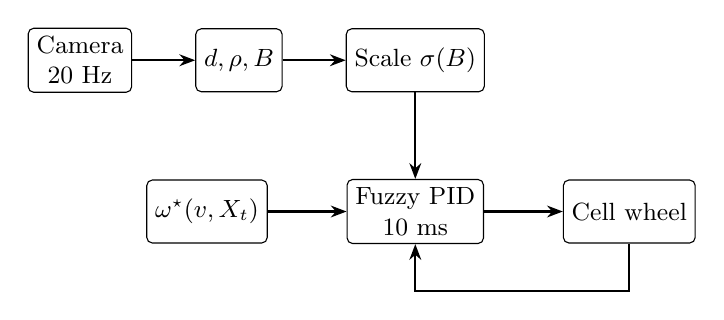
\begin{tikzpicture}[
  font=\small,
  box/.style={draw, rounded corners=2pt, align=center, minimum height=8mm, inner sep=3pt},
  arr/.style={-{Stealth[length=2mm]}, thick}
]
\node[box] (cam) {Camera\\20~Hz};
\node[box, right=8mm of cam] (feat) {$d,\rho,B$};
\node[box, right=8mm of feat] (sig) {Scale $\sigma(B)$};
\node[box, below=11mm of sig] (pid) {Fuzzy PID\\10~ms};
\node[box, left=10mm of pid] (law) {$\omega^{\star}(v,X_t)$};
\node[box, right=10mm of pid] (mot) {Cell wheel};
\draw[arr] (cam) -- (feat);
\draw[arr] (feat) -- (sig);
\draw[arr] (sig) -- (pid);
\draw[arr] (law) -- (pid);
\draw[arr] (pid) -- (mot);
\draw[arr] (mot.south) -- ++(0,-6mm) -| (pid.south);
\end{tikzpicture}
\caption{The camera publishes a bridge index. The motor loop tracks a scaled speed command and does not wait for the next frame.}
\end{figure}

A red-oak frame with $\rho=0.62$ and $c_d=0.15$ gives $B=0.48$ and a scale of 0.965, so 22.0~r/min becomes 21.2~r/min. A bur-oak frame with $\bar d=32$~mm and $\rho=0.70$ hits the cap and falls to 17.2~r/min. The first case should barely intervene. The second gives large seeds more time. Whether that time becomes filled cells depends on vibration as well as on the wheel, which this paper does not control.

\section{Inner loop}

The design model of the loaded wheel motor is $0.18\dot\omega+\omega=u$. The sample is 10~ms. The discrete law is a fuzzy proportional--integral--derivative controller with nominal gains $K_p=2.4$, $K_i=6.0$, and $K_d=0.08$, plus bounded increments from a five-label Mamdani table on the scaled error and its difference \cite{mamdani1974,zadeh1965,astrom2006}. Integral action freezes when the error exceeds 0.8~rad/s or the command is on its rail, which is the integral separation used by He and colleagues to limit overshoot \cite{he2017}. The derivative path is filtered at 40~Hz. Frozen gains stay positive inside the increment box, so each frozen loop is an ordinary stable speed servo. That is not a Lyapunov certificate for the time-varying fuzzy system. The schedule moves with the tracking error, and the error of a 0.18~s plant does not cross the linguistic range in one sample unless the setpoint jumps. Jumps are rate-limited.

Shaft speed is a windowed difference over eight samples, 80~ms, so a 4096-count encoder does not dominate the fuzzy input. A cell at 22~r/min arrives every 0.228~s. Vision samples the throat about four times per cell, which is the point of looking at the throat rather than at the tube: the constraint can act on the cell that is about to be filled. Four frames at a 30~ms abort budget still fit inside that cell period. They stop fitting near 2.1~m/s, which is outside the specified speed and is the same class of limit Borja observed.

\section{What the estimate shows}

Spacings were generated from the logistic event model of the parent thesis, 4{,}000 cells per case, generator seed 20261029. Quality of feed, multiple index, and miss index follow Kachman and Smith: spacings in $(0.5X_t,1.5X_t]$, at most $0.5X_t$, and above $1.5X_t$ \cite{kachman1995}. Planting efficiency is qualified spacings per second divided by $v/X_t$. The vision mode is electronic tracking plus Equation~\eqref{eq:sigma}. Factors stay at a fixed zero shaker frequency and 3~kPa of assist vacuum, so this column is the feed controller alone.

\begin{table}[ht]
\centering
\caption{Vision against speed tracking. $Q_{\mathrm{f}}$, multiple, and miss are percentages. $\eta_{\mathrm{E}}$ is planting efficiency.}
\label{tab:v}
\small
\begin{tabular}{@{}llrrrr@{}}
\toprule
Case & Mode & $Q_{\mathrm{f}}$ & Mult. & Miss & $\eta_{\mathrm{E}}$ \\
\midrule
Red oak, level, 6~Hz & PID & 60.9 & 22.5 & 16.6 & 61.0 \\
 & Vision & 68.5 & 12.5 & 19.0 & 60.7 \\
Pin oak, level, 6~Hz & PID & 51.8 & 34.3 & 13.9 & 61.6 \\
 & Vision & 60.6 & 24.3 & 15.2 & 63.8 \\
Bur oak, 8$^\circ$, 12~Hz & PID & 30.2 & 12.7 & 57.1 & 11.9 \\
 & Vision & 30.2 & 5.6 & 64.1 & 9.8 \\
Red oak, level, 16~Hz & PID & 36.9 & 21.2 & 41.9 & 21.8 \\
 & Vision & 41.1 & 13.2 & 45.6 & 22.0 \\
\bottomrule
\end{tabular}
\end{table}

On mild red oak the multiple index falls by about ten points and the miss index rises by about two. Efficiency does not move. The constraint removes doubles and pays with longer gaps. On pin oak, where the cell is large for the seed, multiples fall from 34.3\% to 24.3\% and efficiency rises only two points. On bur oak in slope and a 12~Hz disturbance, efficiency falls from 11.9\% to 9.8\% and the miss index rises. Under a 16~Hz disturbance on red oak, doubles fall and misses rise, and efficiency stays near 22\%. Slowing a meter that is missing because of vibration creates longer gaps. The feed controller is not a substitute for a vibrator or a depth loop.

These figures are solutions of a declared model anchored to published qualitative facts: slip hurts a ground drive, vision can cut misses when the computer keeps up, and large hardwood seeds defeat a fixed cell \cite{wells1990,zhao2024,borja2021}. They are not belt measurements. A sticky-belt comparison of the PID and vision rows is the acceptance test. The ranking to look for is a lower multiple index on red oak and pin oak, and no requirement that vision alone raise efficiency when the frame is shaking above about 10~Hz.

\section{Spacing side effect and faults}

A constant scale $\sigma$ stretches the geometric gap from $X_t$ to $X_t/\sigma$. At the cap, $\sigma=0.78$, every gap grows by a factor of about 1.28 if the cells that do fill are singles. Part of that stretch replaces a double. Part of it becomes a miss if the next cell was going to be empty anyway. The efficiency column in Table~\ref{tab:v} is that second part. A score that looked only at doubles would drive $\sigma$ to the floor. The cap, and the separate efficiency number, are what stop that.

The feed computer has four local faults. A late vision message holds $B$. After 150~ms, $B$ decays and the constraint opens while tracking continues. Two missed shaft-encoder periods remove motor current. A stale ground speed is held for one second and then ramped to zero, so a dead radar does not leave the wheel planting forever. A radar stuck at a high value is not detected by these rules. It looks like a healthy, fast tractor. That case needs a second speed source before it can be tripped. None of the four faults asks the factor coordinator for help. The camera can fail and the shaft loop remains a speed servo at $\sigma=1$.

\section{Conclusion}

The feed-speed controller is a cascade with one extra scalar. Equation~\eqref{eq:w} sets the speed of a clear throat. Equation~\eqref{eq:sigma} reduces that speed when Equation~\eqref{eq:B} says the throat is bridging, and the reduction is capped. The motor loop does not decode images. The estimate says the scalar does what it was built to do: it cuts doubles on seeds that nearly fit the cell, and it does not, by itself, recover bur oak or a harshly vibrating frame. Planting efficiency must be reported beside the quality-of-feed index, because a controller scored only on doubles will always prefer the lowest scale.

\begin{thebibliography}{10}
\bibitem{lof2019} M.~L\"of et al., ``Tamm Review: Direct seeding to restore oak forests and woodlands,'' \emph{Forest Ecol.\ Manage.}, vol.~448, pp.~474--489, 2019.
\bibitem{he2017} X.~He et al., ``Design and evaluation of a PID electronic control system for seed meters,'' \emph{Trans.\ CSAE}, vol.~33, no.~17, pp.~28--33, 2017.
\bibitem{zhao2024} X.~Zhao et al., ``Electronic control seed-metering system based on fuzzy PID,'' \emph{Int.\ J.\ Agric.\ Biol.\ Eng.}, vol.~17, no.~4, 2024.
\bibitem{kocher1998} M.~F.~Kocher, Y.~Lan, C.~Chen, and J.~A.~Smith, ``Opto-electronic sensor system for rapid evaluation of planter seed spacing uniformity,'' \emph{Trans.\ ASAE}, vol.~41, no.~1, pp.~237--245, 1998.
\bibitem{borja2021} A.~A.~Borja, R.~M.~Amongo, J.~P.~Pabico, and D.~C.~Suministrado, ``A machine vision system and mechatronic drive for a pneumatic seed meter,'' \emph{Philipp.\ J.\ Agric.\ Biosyst.\ Eng.}, vol.~17, no.~1, 2021.
\bibitem{otsu1979} N.~Otsu, ``A threshold selection method from gray-level histograms,'' \emph{IEEE Trans.\ Syst., Man, Cybern.}, vol.~9, no.~1, pp.~62--66, 1979.
\bibitem{mamdani1974} E.~H.~Mamdani, ``Application of fuzzy algorithms for control of a simple dynamic plant,'' \emph{Proc.\ IEE}, vol.~121, no.~12, pp.~1585--1588, 1974.
\bibitem{zadeh1965} L.~A.~Zadeh, ``Fuzzy sets,'' \emph{Inf.\ Control}, vol.~8, no.~3, pp.~338--353, 1965.
\bibitem{astrom2006} K.~J.~{\AA}str\"om and T.~H\"agglund, \emph{Advanced PID Control}. ISA, 2006.
\bibitem{kachman1995} S.~D.~Kachman and J.~A.~Smith, ``Alternative measures of accuracy in plant spacing,'' \emph{Trans.\ ASAE}, vol.~38, no.~2, pp.~379--387, 1995.
\bibitem{wells1990} L.~G.~Wells, T.~W.~Richards, T.~D.~Smith, and G.~B.~Day, ``Pneumatic metering of hardwood tree seeds,'' \emph{Appl.\ Eng.\ Agric.}, vol.~6, no.~2, pp.~239--243, 1990.
\end{thebibliography}

\end{document}
